\documentclass[border=2pt]{standalone}
\usepackage{tikz}
\begin{document}
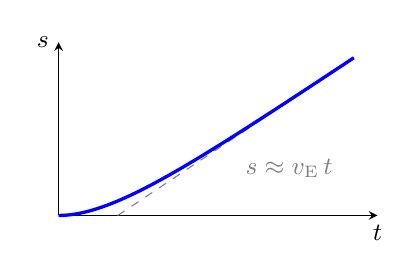
\begin{tikzpicture}[>=stealth, font=\small, xscale=0.75, yscale=0.5]
 \draw[->] (0,0) -- (5.4,0) node[below] {$t$};
 \draw[->] (0,0) -- (0,4.4) node[left] {$s$};
 \draw[dashed, gray] (1,0) -- (5,4);
 \draw[blue, very thick, domain=0:5, samples=60] plot (\x, {\x-1+exp(-\x)});
 \node[gray, anchor=west] at (3.0,1.2) {$s \approx v_\mathrm{E}\,t$};
\end{tikzpicture}

\medskip
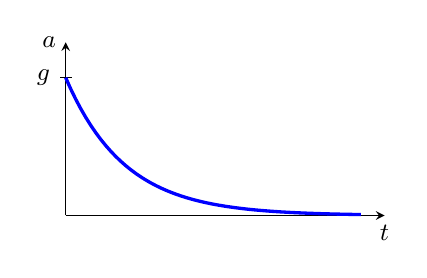
\begin{tikzpicture}[>=stealth, font=\small, xscale=0.75, yscale=0.5]
 \draw[->] (0,0) -- (5.4,0) node[below] {$t$};
 \draw[->] (0,0) -- (0,4.4) node[left] {$a$};
 \draw (0.1,3.5) -- (-0.1,3.5) node[left] {$g$};
 \draw[blue, very thick, domain=0:5, samples=60] plot (\x, {3.5*exp(-\x)});
\end{tikzpicture}
\end{document}
